% =====================================================================
% ECE 510 -- HW4AI -- Milestone 4 Design Justification Report
% Build:  make            (runs pdflatex twice for refs)
%         make clean
%
% This is a FILLABLE TEMPLATE.
%   - Yellow boxes  (\question{...}) flag input the author must supply;
%     search for "QUESTION" or "\question" to find them all.
%   - Red text      (\fillin{...}) marks short blanks to replace.
%   - Sections pre-filled from the repo (synthesis/benchmark numbers,
%     "what did not work") are factual and traceable; verify and keep.
%   - Target length: ~2000-2500 words (closer to 2000 than 5000).
%   - Delete the "How to use" and "Open questions" boxes before final.
% =====================================================================
\documentclass[11pt]{article}

\usepackage[letterpaper,margin=1in]{geometry}
\usepackage{graphicx}
\usepackage{xcolor}
\usepackage{amsmath}
\usepackage{booktabs}
\usepackage{enumitem}
% (Optional) clickable cross-references: add \usepackage[hidelinks]{hyperref}.
% Left out by default so the report builds on minimal TeX installs too.

% Render the text underscore as a plain rule (OT1/Computer Modern) instead of
% the TS1 companion glyph. Keeps the doc buildable on minimal TeX installs
% that lack Metafont / scalable TS1 fonts; harmless on a full TeX Live. If you
% prefer the nicer TS1 underscore, delete this and add \usepackage{lmodern}.
\newcommand{\ruleunderscore}{\leavevmode\kern0.04em\vbox{\hrule width0.32em height0.4pt}\kern0.04em}
\AtBeginDocument{\renewcommand{\_}{\ruleunderscore}\renewcommand{\textunderscore}{\ruleunderscore}}

% ---- author-input helpers (remove the boxes before final submit) ----
\newcommand{\question}[1]{%
  \par\medskip\noindent
  \colorbox{yellow!35}{\parbox{\dimexpr\linewidth-2\fboxsep\relax}{%
  \textbf{\textcolor{red!60!black}{QUESTION FOR AUTHOR:}} #1}}\par\medskip}
\newcommand{\fillin}[1]{\textcolor{red}{\textbf{[#1]}}}

\title{\vspace{-2em}Custom Systolic-Array Accelerator for RAFT Convolution\\
       \large ECE 510 / HW4AI -- Milestone 4 Design Justification}
\author{Elliott Day}
\date{\today}

\begin{document}

% --------------------------- title page ----------------------------
\begin{titlepage}
\centering
\IfFileExists{figures/psu_logo.png}{%
  
\includegraphics[width=0.55\textwidth]{figures/psu_logo.png}\par\vspace{1.6cm}}{%
  \fbox{\parbox{0.6\textwidth}{\centering\vspace{1cm}
  \textbf{[ Portland State University logo ]}\\[0.3em]
  \footnotesize place the official PNG at \texttt{figures/psu\_logo.png}
  \vspace{1cm}}}\par\vspace{1.6cm}}

{\Large\bfseries Custom Systolic-Array Accelerator for RAFT Convolution\par}
\vspace{0.5cm}
{\large Milestone 4 -- Design Justification Report\par}
\vspace{0.3cm}
{\large ECE 510: Hardware for AI and Machine Learning\par}
\vspace{2.5cm}

{\Large Elliott Day\par}
\vspace{0.4cm}
{\large Portland State University\par}
\vspace{0.3cm}
{\normalsize Spring 2026 \quad\textbar\quad \today\par}

\vfill
{\small 16$\times$16 weight-stationary systolic array, bf16$\times$bf16$\rightarrow$fp32,
100\,MHz, sky130 (OpenLane 2).\par}
\end{titlepage}

% ----------------------- how-to + open questions --------------------
\noindent\colorbox{yellow!20}{\parbox{\dimexpr\linewidth-2\fboxsep\relax}{%
\textbf{How to use this template (delete before final).} Replace every
\fillin{red blank} and answer every \textbf{\textcolor{red!60!black}{QUESTION
FOR AUTHOR}} box, then remove this box and the list below. Keep the nine
section headings exactly as-is (the grader counts them). Aim for 2000--2500
words total. Build with \texttt{make}.}}

\question{Optional polish only: all required sections are filled (name,
precision, diagrams, verification, synthesis, benchmark, what-did-not-work).
Add anything in Sec.~1 about the end application you want to emphasize, then
delete the boxes above before submitting.}

\begin{abstract}
\noindent
This report documents a custom hardware accelerator for the dominant
convolution kernel of the RAFT \texttt{raft\_large} optical-flow network.
The design is a 16$\times$16 weight-stationary systolic array (256
multiply-accumulate cells) using bf16 multiplication with fp32 accumulation,
wrapped in an AXI4-Stream data plane and an AXI4-Lite control plane. It is
verified in cocotb co-simulation and pushed through the OpenLane~2 / sky130
flow, closing timing at 100\,MHz (worst setup slack +0.667\,ns) with an
estimated 0.834\,W and 16.38\,mm$^2$ die. Benchmarked against the M1 CPU
software baseline on the target layer, the accelerator is currently
memory/reload bound (effective arithmetic intensity 0.92 FLOP/byte) and does
\emph{not} beat the CPU on this layer. The shortfall is a planning gap -- a
per-tile weight-reload schedule that I did not integration-test until late --
not a datapath defect; this report analyzes the root cause, the streaming fix I
prototyped, and why it was deferred.
\end{abstract}

% =====================================================================
\section{Problem and motivation}
% =====================================================================
This project accelerates RAFT (Recurrent All-Pairs Field Transforms), a
learned optical-flow network, with the target application being
machine-learning-based SLAM front-ends for edge robotics. Learned-SLAM
front-ends built on RAFT-style flow and correspondence are accurate but, on a
GPU, power-hungry and physically bulky; while GPUs and accelerators exist for
related learned-SLAM kernels, there is no RAFT-specific hardware. The goal is
to run the same workload inside an edge power/area budget at real-time rates
(30--60\,fps), trading the GPU's generality for efficiency on this one network.

Two properties make RAFT a good custom-silicon target. First, it is
\textbf{convolution-dominated}: M1 profiling of \texttt{raft\_large}
(\texttt{project/m1/sw\_baseline.md}, \texttt{codefest/cf02/profiling}) found
2D convolution (\texttt{aten::mkldnn\_convolution}) to be the dominant cost at
\textbf{53.02\%} of forward self-CPU time, on a mean forward of
\textbf{4.145\,s} and \textbf{788.14\,GMAC} per forward. Second, it
\textbf{tolerates reduced precision}: the M2 analysis (Sec.~3) shows bf16
multiply with fp32 accumulate meets an engineering error bound, so the
area-dominant multipliers can be small. A weight-stationary systolic array
exploits convolution's regular multiply-accumulate structure and weight reuse
directly in silicon, motivating a custom datapath rather than a
general-purpose core.

The original proposal targeted a 48$\times$48 array; the delivered scope is a
16$\times$16 array at 100\,MHz (Sec.~7 explains the scope reduction). The rest
of this report characterizes that design and is candid about where it falls
short of the real-time goal (Sec.~8--9).

% =====================================================================
\section{Roofline analysis}
% =====================================================================
The target layer (\texttt{Conv2d 5-1}, \(C_{in}{=}C_{out}{=}64\), \(3\times3\),
batch~4, \(260\times480\)) has \(\sim\)36.9\,GFLOP. With fp32 operands and no
reuse its intrinsic arithmetic intensity is \(\sim\)144 FLOP/byte. The
accelerator's compute roof is \(256\times2\times100\,\text{MHz}=51.2\)
GFLOP/s; its binding memory roof is the AXI4-Stream pin bandwidth
(one 256-bit beat/cycle at 100\,MHz \(=3.2\) GB/s), giving a ridge point at
\(\text{AI}^{*}=16\) FLOP/byte. As built, the schedule reloads the weight
slab on every K-tile and reuses resident weights across zero extra pixels, so
the \emph{measured} effective AI collapses to \textbf{0.92 FLOP/byte} --
deep in the memory/reload-bound region (Fig.~\ref{fig:roofline}).

The design is memory-bottlenecked in a way I did not anticipate, and the cause
is a planning gap rather than a single bad gate. Because weights are reloaded
per tile, the weight-streaming cost grows steeply with the number of pixels
that must be convolved, and that weight movement -- not the 256 MAC/cycle the
array can sustain -- ends up dominating runtime. The two fixes I identified
are to enlarge the on-chip weight store and to stream a block of pixel-columns
through each resident weight set so one load is amortized over many pixels
(Sec.~4); I attempted the streaming version but hit further LibreLane/PnR
issues (Sec.~9) and shipped this flawed-but-closing design instead. The central
architectural lesson stands: the dataflow's reuse, not the array's peak, sets
delivered performance.

\begin{figure}[t]
\centering
\IfFileExists{../bench/roofline_final.png}{%
  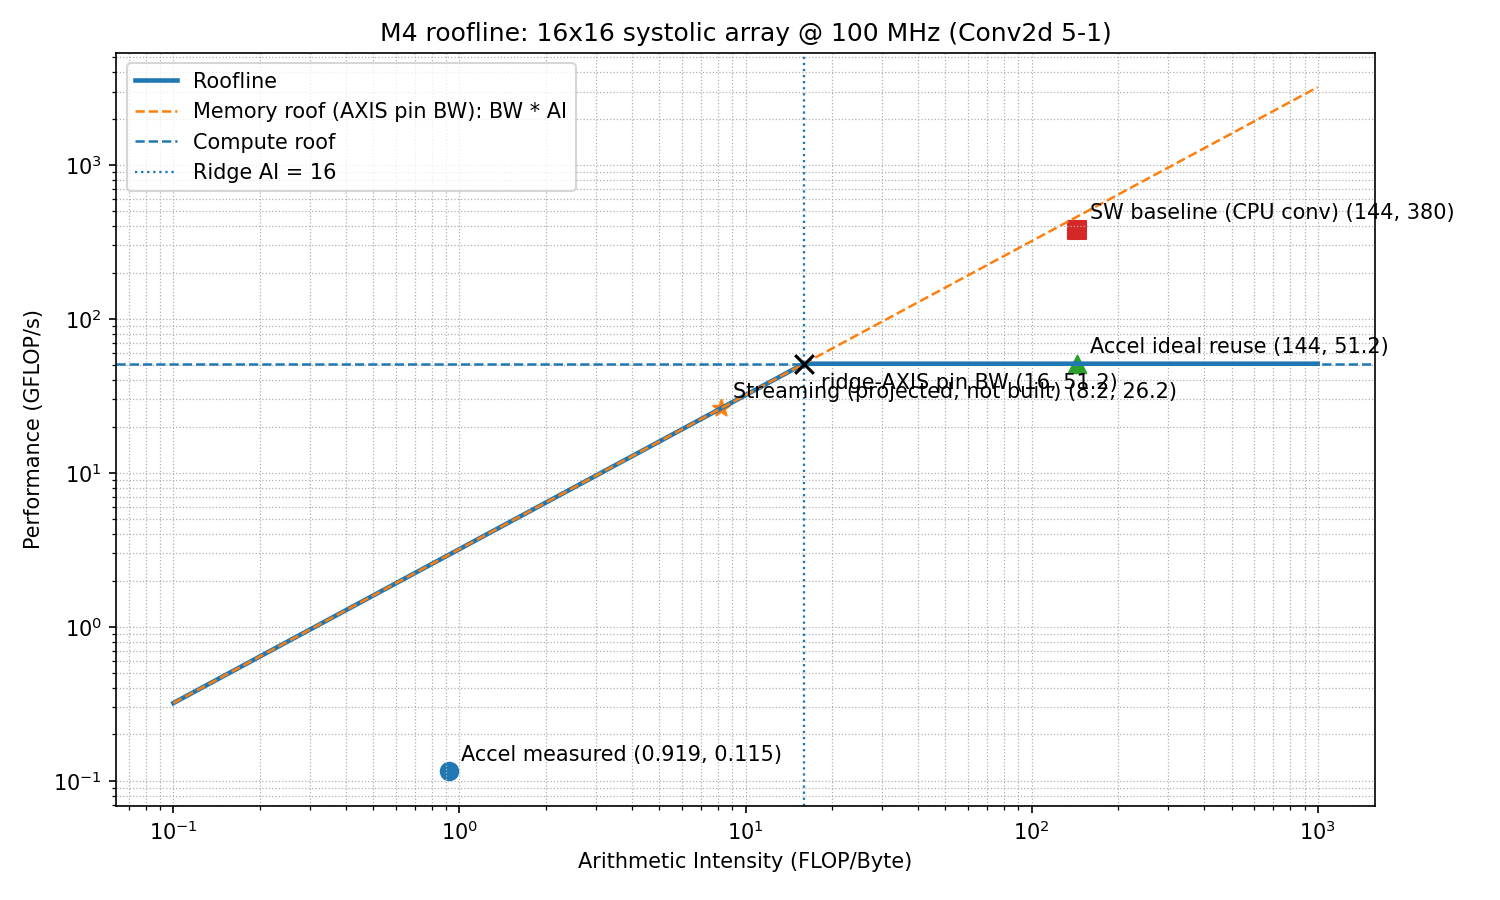
\includegraphics[width=0.85\textwidth]{../bench/roofline_final.png}}{%
  \fbox{\texttt{../bench/roofline\_final.png missing -- run tools/roofplot}}}
\caption{Roofline for the 16$\times$16 array (compute roof 51.2 GFLOP/s, pin
bandwidth 3.2 GB/s, ridge AI = 16). The measured operating point sits at
AI 0.92, 0.115 GFLOP/s; the CPU software baseline and the (not-built)
streaming projection are shown for context.}
\label{fig:roofline}
\end{figure}

% =====================================================================
\section{Precision and data format}
% =====================================================================
The datapath multiplies two bf16 operands, accumulates in fp32 across the
K-reduction, and drains the result back to bf16 (round-toward-zero) on output;
subnormal inputs flush to signed zero. The product of two normal bf16 values is
exact in the fp32 mantissa, so the only rounding sources are the fp32 adds and
the final bf16 drain. bf16 keeps the 8-bit exponent of fp32 (same dynamic
range) while shrinking the multiplier mantissa to 8$\times$8 -- the dominant
area term -- and fp32 accumulation avoids the fp16-style creep that would
otherwise build over the long convolution inner products.

I validated this in M2 (\texttt{project/m2/precision.md}) with a Gaussian
stress sweep (\texttt{tb/tb\_quant\_error.py}): \texttt{SEED=42}, 30 tiles
$\rightarrow$ \textbf{1440} bf16 outputs, four times the 100-sample rubric
minimum, run on the headline 48$\times$48 array so the reduction depth
($K{=}48$) is deeper than -- and bounds -- the shipped 16$\times$16 tile. The
hardware was compared against a software model that round-trips through fp32
after every multiply and add (tracking fp32, not fp64). Measured error:
\textbf{MAE $=4.87\times10^{-2}$}, RMSE $6.28\times10^{-2}$, max abs error
$2.70\times10^{-1}$. The dominant error bin $[10^{-2},10^{-1})$ is the expected
$\sqrt{K}$ growth as reduction depth rises, and the dimensionless
$\text{MAE}/\sqrt{\mathrm{Var}(y)}$ stays small.

I declare an \textbf{engineering pass} when MAE $<10^{-1}$ against this
stimulus; the measured $4.87\times10^{-2}$ clears it with $\sim$2$\times$
margin. The acceptability ceiling is tied to the end task: RAFT reports
KITTI/Sintel end-point error at the sub-pixel to few-pixel scale, so feature
noise at MAE $<5\times10^{-2}$ is small relative to the iterative refinement
and motion magnitudes that dominate the benchmark. (Round-toward-zero adds a
small one-sided bias on long dot products; switching the accumulate/drain to
round-to-nearest-even is the documented precision follow-up.)

% =====================================================================
\section{Dataflow and architecture}
% =====================================================================
The top-level structure (Fig.~\ref{fig:block}) is a bus-pin-only wrapper: an
AXI4-Stream ingress FIFO feeds a one-bit \texttt{cfg\_mode} demux that routes
each beat either to \texttt{weight\_store} (LOAD) or to the compute core
(COMPUTE); \texttt{load\_seq} replays the stored weights into the PE array; and
results return through an egress FIFO and a registered \texttt{skid\_buffer} to
the AXI4-Stream master. An \texttt{interface\_module} (AXI4-Lite) supplies
\texttt{cfg\_start/mode/accum/hold} and reports \texttt{status\_busy/done}.

\begin{figure}[t]
\centering
\IfFileExists{figures/block_diagram.png}{%
  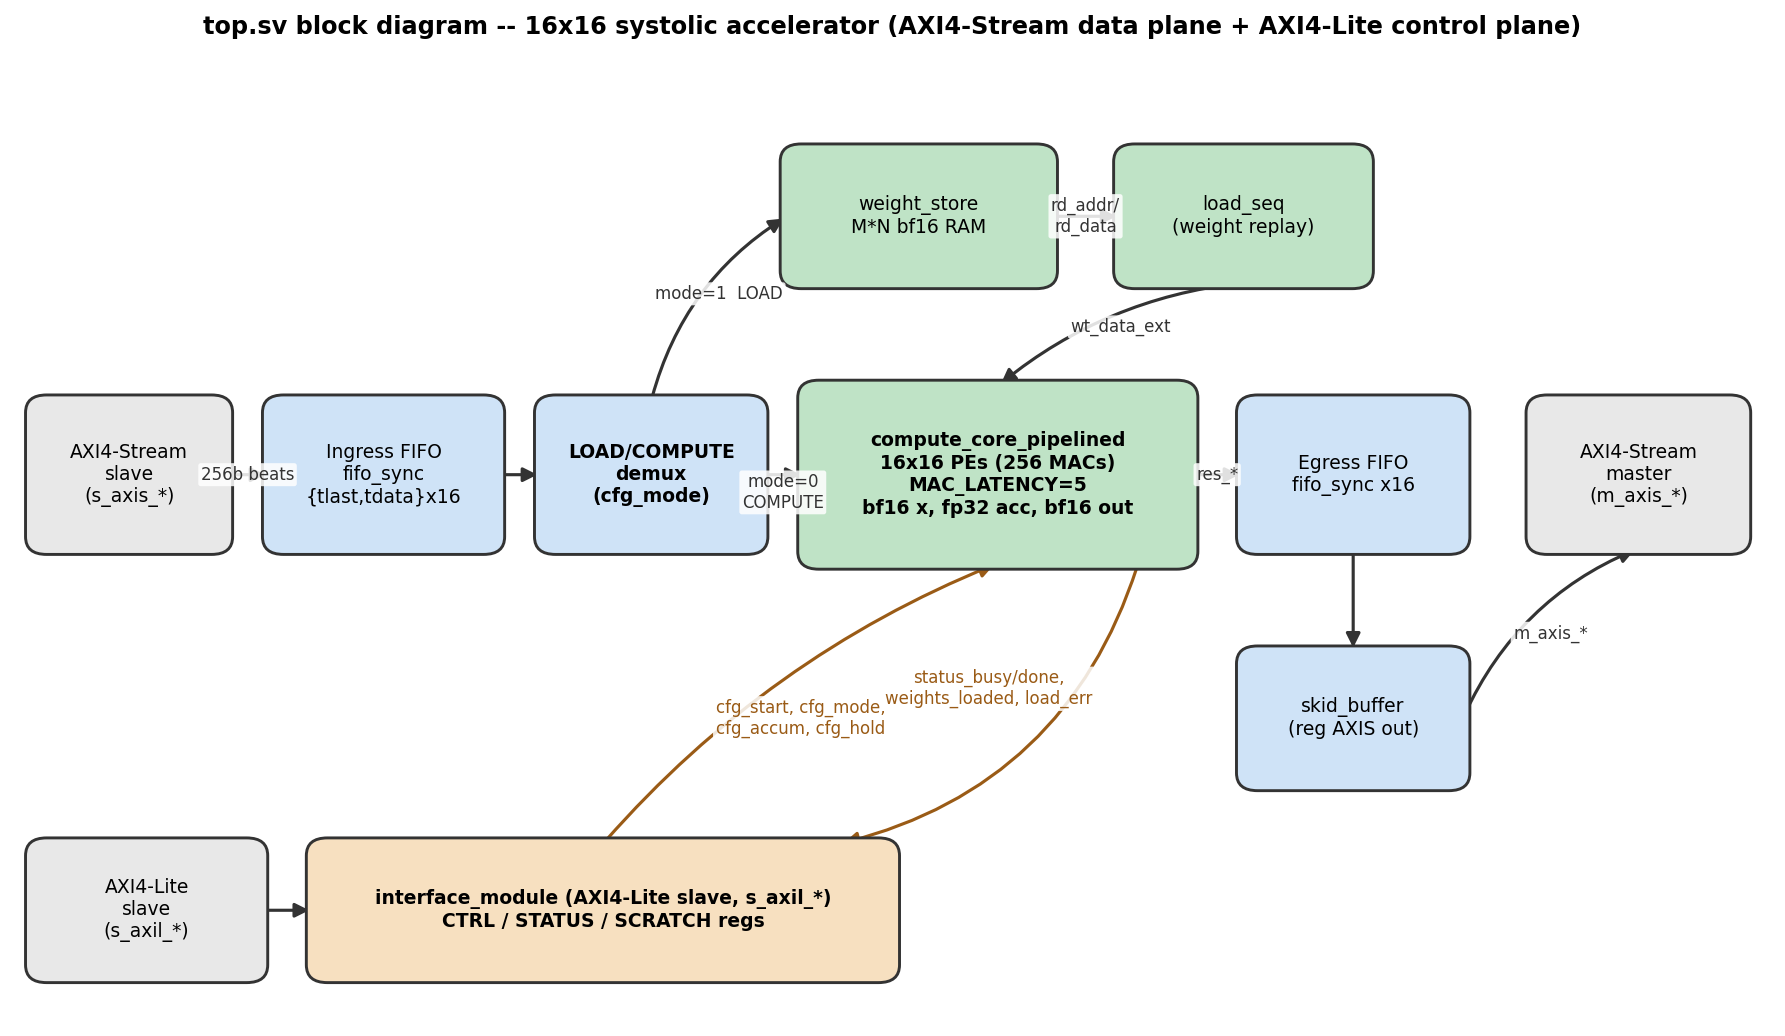
\includegraphics[width=\textwidth]{figures/block_diagram.png}}{%
  \fbox{\texttt{figures/block\_diagram.png missing -- run make\_block\_diagram.py}}}
\caption{\texttt{top.sv} block diagram: AXI4-Stream data plane (ingress FIFO,
LOAD/COMPUTE demux, \texttt{weight\_store} + \texttt{load\_seq}, compute core,
egress FIFO, skid buffer) and AXI4-Lite control plane.}
\label{fig:block}
\end{figure}

The array is \textbf{weight-stationary}: a 16$\times$16 tile of weights is
loaded into the 256 PEs and held while activations stream through, so each
weight is read once per tile and reused across the activation columns fed
during that tile (Fig.~\ref{fig:dataflow}). Each PE performs one bf16 multiply
and one fp32 add per cycle (\texttt{pe\_pipelined.sv}, \texttt{mul\_bf16\_p2},
\texttt{add\_fp32\_p2});
results reduce down each column into 16 fp32 accumulators
(\texttt{result\_buf}). A LOAD/COMPUTE/DRAIN FSM (\texttt{compute\_core\_pipelined.sv})
sequences weight load, activation streaming with the pipeline skew
(\texttt{MAC\_LATENCY}), and result drain; \texttt{weight\_store} and
\texttt{load\_seq} stage the weight slab, and two synchronous FIFOs buffer the
AXI-Stream ingress/egress. Weight-stationary fits convolution because the same
filter weights apply across many output pixels -- though, as Sec.~2 notes, the
\emph{current} tile schedule does not exploit that cross-pixel reuse.

The architectural weakness is here: the tile schedule reloads the full weight
slab for every K-tile, so the weight-load cycles scale with the pixel count
rather than amortizing across it, and weight streaming becomes the runtime
bottleneck. I have two RTL changes would help close the gap. First, enlarging the
\texttt{weight\_store} so more of the filter bank stays resident reduces how
often the slab is reloaded. Second streaming a block of
$B$ pixel-columns through each resident weight set amortizes one weight load
over $B$ pixels, raising effective AI by roughly the block factor. I prototyped
the streaming path but could not get it through PnR in the time available
(Sec.~9), so the shipped design keeps the simpler per-pixel schedule.

\begin{figure}[t]
\centering
\IfFileExists{figures/dataflow_diagram.png}{%
  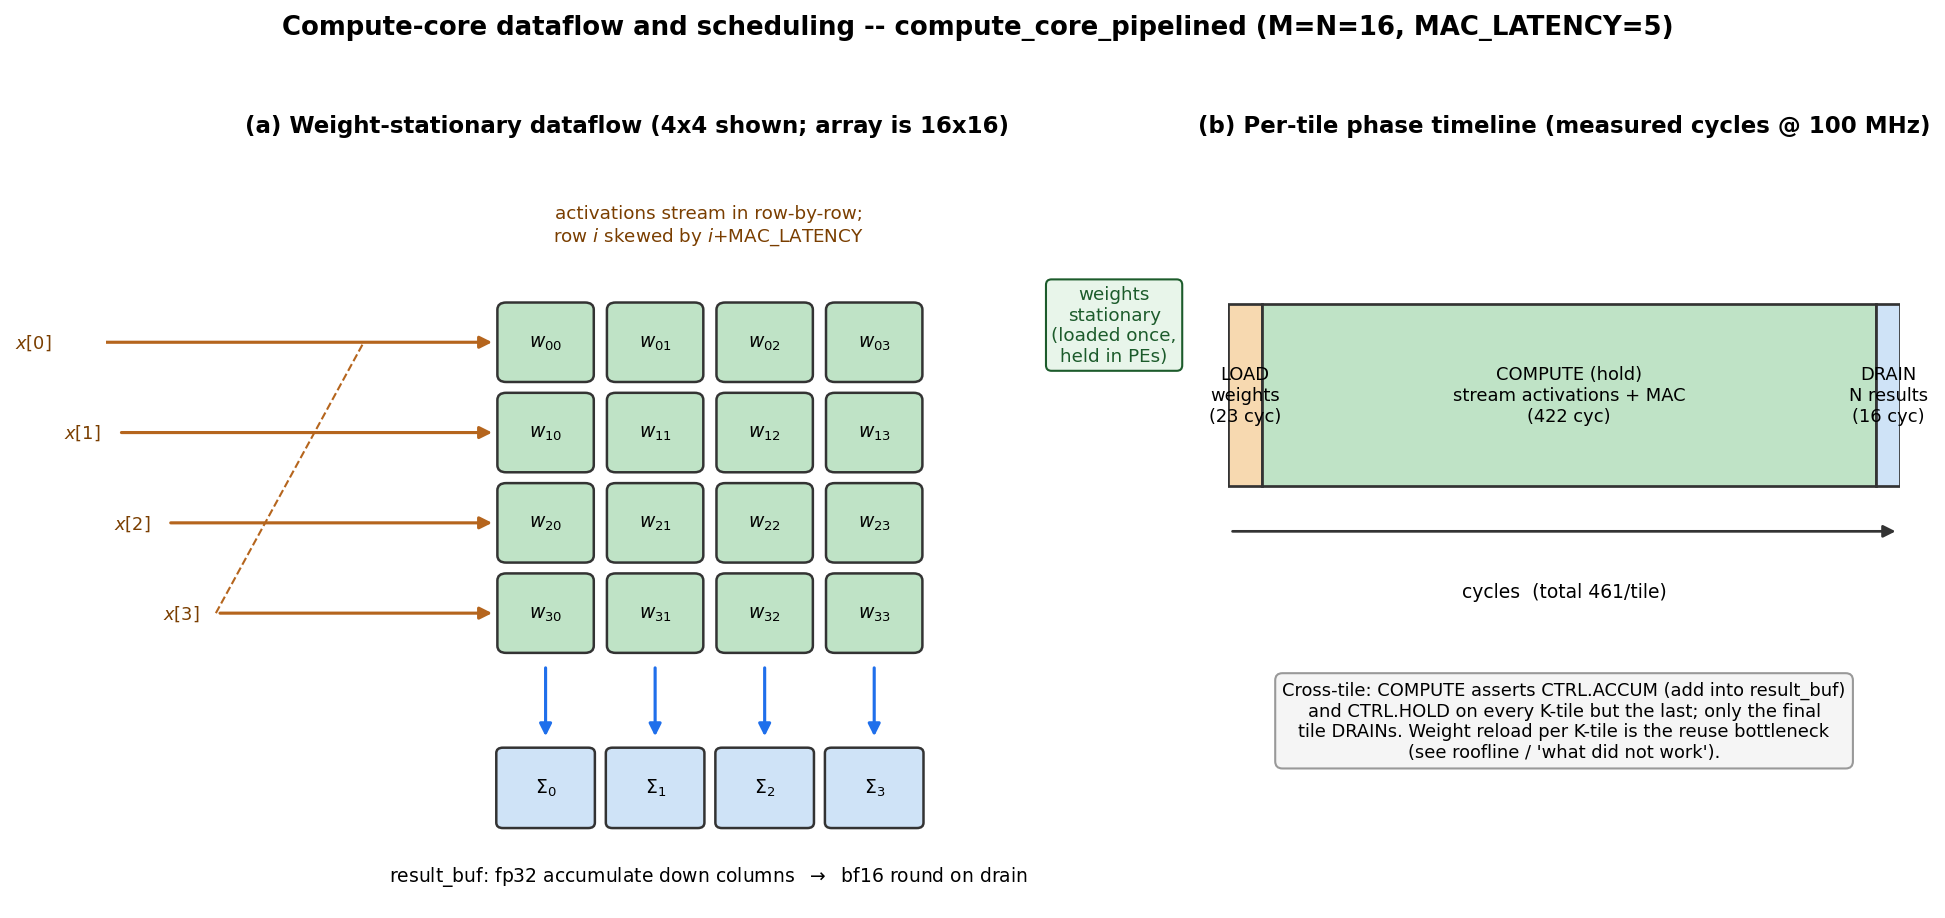
\includegraphics[width=\textwidth]{figures/dataflow_diagram.png}}{%
  \fbox{\texttt{figures/dataflow\_diagram.png missing -- run make\_dataflow\_diagram.py}}}
\caption{Compute-core dataflow. (a) Weights stay resident in the PE grid while
activations enter row-by-row with the \texttt{MAC\_LATENCY}=5 skew and partial
products accumulate down each column in fp32, rounding to bf16 only on drain.
(b) The per-tile LOAD/COMPUTE(hold)/DRAIN phase timeline with measured cycle
counts; cross-K tiles use \texttt{CTRL.ACCUM}/\texttt{HOLD} and only the last
tile drains.}
\label{fig:dataflow}
\end{figure}

% =====================================================================
\section{Hardware interface}
% =====================================================================
The data plane is \textbf{AXI4-Stream} (256-bit \texttt{tdata}) and the control
plane is \textbf{AXI4-Lite} (host writes mode/start, polls status). AXI4-Stream
was chosen in M1 (\texttt{project/m1/interface\_selection.md}) for high-throughput
bulk tensor streaming. At 100\,MHz the stream delivers 3.2\,GB/s of pin
bandwidth. The design is \textbf{interface/bandwidth bound} at the current
operating point: at AI 0.92 FLOP/byte the 3.2\,GB/s roof caps performance near
2.9 GFLOP/s, and the reload-stalled schedule delivers even less (0.115
GFLOP/s, see Sec.~8). The array's 51.2 GFLOP/s compute capability is therefore
not the limiter -- data movement is.

% =====================================================================
\section{Verification}
% =====================================================================
Correctness was verified by cocotb co-simulation (\texttt{tb/tb\_top.py}),
driving the DUT \emph{only} through its AXI pins -- no internal compute-core
probes -- and checking every output against an \emph{independent} software
reference (bf16-accurate or fp64), never a prior DUT run. The default run is
\textbf{6 PASS + 2 skipped} (the two opt-in cases run under environment flags);
\texttt{sim/cosim\_run.log} and \texttt{tb/results.xml} record the contract:

\begin{itemize}[noitemsep,topsep=2pt]
  \item \texttt{test\_top\_smoke} -- after reset, all bus outputs sit at sane
        idle values.
  \item \texttt{test\_axil\_scratch\_loopback} -- AXI4-Lite write/read of the
        SCRATCH register, proving the control path before anything depends on
        it.
  \item \texttt{test\_gemm\_tile\_e2e} (headline) -- one im2col$\rightarrow$GEMM
        tile of the M1 dominant kernel: load the $M\times N$ weight slab, run a
        COMPUTE tile, and check all $N$ outputs bit-exact against the bf16
        reference.
  \item \texttt{test\_weight\_reuse\_two\_activation\_tiles} -- load weights
        once, run two activation tiles with no second weight push; a broken
        weight cache would stall and time out.
  \item \texttt{test\_backpressure} -- hold \texttt{m\_axis\_tready}=0 for 6
        cycles after the first beat and confirm the remaining $N{-}1$ results
        still arrive bit-exact, exercising the AXIS handshake and the egress
        FIFO decoupling.
  \item \texttt{test\_conv\_e2e} -- end-to-end tiled convolution with
        \emph{hardware} cross-tile fp32 accumulation (\texttt{CTRL.ACCUM}/%
        \texttt{HOLD}), sweeping $K$ in $M$-deep slices and comparing every
        output pixel/channel bit-exact to an fp64 convolution reference.
  \item Opt-in: \texttt{test\_conv\_raft\_dims\_e2e}
        (\texttt{RUN\_RAFT\_DIMS}, $C_{in}{=}C_{out}{=}64$, $3\times3$) and
        \texttt{test\_benchmark} (\texttt{RUN\_BENCH}, measures the per-phase
        cycle counts used in Sec.~8).
\end{itemize}

Together these cover the control path, the AXIS handshake under backpressure,
single-tile GEMM correctness (bf16 multiply / fp32 accumulate / bf16 round),
weight-cache reuse, and multi-tile convolution accumulation.
Figure~\ref{fig:waveform} shows a representative co-simulation waveform.

\begin{figure}[t]
\centering
\IfFileExists{../sim/cosim_waveform.png}{%
  
\includegraphics[width=\textwidth]{../sim/cosim_waveform.png}}{%
  \fbox{\texttt{../sim/cosim\_waveform.png missing -- run sim/render\_waveform.py}}}
\caption{Co-simulation waveform of a GEMM tile through the AXI pins
(\texttt{sim/render\_waveform.py}): the LOAD/COMPUTE handshake, activation
streaming, and result drain.}
\label{fig:waveform}
\end{figure}

% =====================================================================
\section{Synthesis results}
% =====================================================================
Synthesis and PnR used OpenLane~2 / sky130
(\texttt{RUN\_2026-06-04\_17-46-11}); numbers below are the post-global-route
signoff snapshot (step 42, typical corner). The run entered detailed routing
but did not finish it (see Sec.~9); step-42 STA is the timing snapshot.

\begin{table}[h]
\centering
\begin{tabular}{lll}
\toprule
Metric & Value & Dominant contributor \\
\midrule
Clock / timing & 100\,MHz, setup MET +0.667\,ns (0 setup vio) & reg-to-reg +1.518\,ns \\
Hold & $-0.969$\,ns WNS, 35 vio & IO-port paths only (reg-to-reg clean) \\
Die area & 16.38\,mm$^2$ (std-cell 8.43\,M\,$\mu$m$^2$) & combinational $\sim$54\% \\
Power (static est.) & 0.834\,W & sequential 48.8\%, clock 36.6\% \\
\bottomrule
\end{tabular}
\caption{Synthesis signoff summary (\texttt{synth/timing\_report.txt},
\texttt{area\_report.txt}, \texttt{power\_report.txt}).}
\label{tab:synth}
\end{table}

The dominant area contributor is combinational logic ($\sim$54\% of placed
std-cell area): the bf16 multipliers and fp32 adders replicated across 256 PEs.
Power is dominated by the $\sim$96.6k async-reset flops (48.8\%) and the clock
network (36.6\%), as expected for a flop-heavy systolic array. The power figure
is OpenROAD's \emph{static} activity estimate, not VCD-back-annotated; the
relative split (sequential $\gg$ clock $\gg$ combinational) is the reliable
takeaway.

The 16$\times$16 @ 100\,MHz operating point is a deliberate scope choice. The
array's peak compute (51.2 GFLOP/s) sits below the CPU baseline largely because
of those two numbers -- the array dimensions and the clock. Earlier, larger and
faster configurations turned every iteration into a 20-hour LibreLane run and
left me debugging the flow instead of the design. Scaling back to 16$\times$16
at 100\,MHz let me actually close timing (Table~\ref{tab:synth}) and iterate on
the architecture. Within the constraints of this course project -- limited tool
time and a still-developing PnR workflow --  a smaller
design that closes and is fully characterized is more defensible than a larger
one stuck mid-flow.

% =====================================================================
\section{Benchmark results}
% =====================================================================
Per-phase cycle costs were measured in simulation
(\texttt{bench/bench\_measured.csv}: load 23, compute-hold 422, drain 16
cycles) and extrapolated to the full layer by \texttt{bench/benchmark.py}
(\texttt{benchmark\_data.csv}). At 100\,MHz the layer takes
\textbf{320.2\,s} (sustained \textbf{0.115 GFLOP/s}, 0.22\% of the 51.2
GFLOP/s roof). The M1 CPU baseline runs the same layer in \textbf{0.097\,s}
(380 GFLOP/s effective conv rate), so the kernel speedup is
\textbf{0.0003$\times$} -- the accelerator is roughly \textbf{3{,}300$\times$
slower} on this layer, and slower on energy (267\,J vs 4.36\,J). This is
reported honestly: the gap is architectural, not a clock or array-size issue.
The CPU's BLAS convolution keeps weights resident and reuses them across the
whole output map; the array's tile schedule reloads weights every K-tile and
achieves no pixel reuse, paying DMA and pipeline-fill cost that swamps the 256
MAC/cycle the array can sustain. The measured point even falls below the
3.2\,GB/s bandwidth ceiling because of reload stalls (Fig.~\ref{fig:roofline}).

\paragraph{Why compute-hold scales so badly with pixels.} The cost model is
closed-form over the tile schedule the RTL runs ($K{=}576$ reduction,
$K_T{=}K/M{=}36$ K-tiles, $N_T{=}C_{out}/N{=}4$ N-tiles,
$P{=}\text{batch}\cdot H_{out}\cdot W_{out}{=}499{,}200$ output pixels). One
output pixel needs $K\cdot C_{out}=36{,}864$ MACs, which a 256-MAC/cycle array
could finish in $\approx144$ cycles. The shipped per-pixel schedule instead
spends
\[
  N_T\big[\,K_T\cdot\underbrace{23}_{\text{load}}
          +(K_T-1)\cdot\underbrace{422}_{\text{compute\_hold}}
          +\underbrace{438}_{\text{full}}\,\big]
  = 4\,[\,36\cdot23 + 35\cdot422 + 438\,] = 64{,}144\ \text{cycles/pixel},
\]
a utilization of only $144/64{,}144\approx0.22\%$. Summed over all pixels, the
\texttt{compute\_hold} term alone is
\[
  P\,N_T\,(K_T-1)\cdot 422 \;=\; 2.95\times10^{10}\ \text{cycles}
  \;=\; 295\ \text{s at 100\,MHz} \;\;(\mathbf{92\%}\ \text{of the }320.2\ \text{s}),
\]
versus 16.5\,s of weight loads and 8.7\,s of drains. The 422-cycle hold is
mostly the $(M{+}N{-}1)\cdot\text{MAC\_LATENCY}=155$-cycle systolic
pipeline-fill latency (plus FIFO/handshake overhead): a single 16-wide
activation column produces only $M\cdot N=256$ MACs, so the fill is never
amortized. Weight-stationary pays off only when many activation columns stream
through one resident weight load -- the design streams exactly one, so this
fill latency is re-paid for every pixel and every K-tile. That is the precise
sense in which \texttt{compute\_hold} scales with the pixel count, and it is
what the streaming fix in Sec.~9 targets.

% =====================================================================
\section{What did not work}
% =====================================================================

\textbf{The blindspot (no pixel reuse).} The shipped schedule pins one output
pixel in the N-wide \texttt{result\_buf} and reloads the full weight slab on
every K-tile, reusing each weight set across exactly one pixel. New to the
hardware/software co-design space, I made a process mistake: I assumed that if
the compute datapath was correct, the interface bandwidth would simply be high
enough for the system to run cleanly, so I skipped a full design integration.
The flaw only surfaced when I ran a fully integrated benchmark and saw the
per-tile costs extrapolate to RAFT scale (Sec.~8): AI collapses to 0.92
FLOP/byte, the array runs at 0.22\% utilization, and the design ends up far
slower than the CPU. The lesson is less about one design choice than about
sequencing -- I should have spent more time understanding the kernel and had an
integration plan from the start, so the roofline/reuse analysis gated the
dataflow \emph{before} I invested in datapath timing closure.

\textbf{The attempted fix (streaming GEMM).} The remedy is to keep weights
resident and stream a block of \(B\) pixel-columns through them, amortizing one
weight load over \(B\) pixels. Modeling showed this would raise effective AI
from \(\sim\)0.92 to \(\sim\)8.2 FLOP/byte (\(\sim\)9$\times$) and move the
operating point up the bandwidth roof (still memory-bound, but far faster). I
implemented a register-based version (\texttt{act\_block[B][M]},
\texttt{result\_buf[B][N]}, a \texttt{PIX\_BLOCK} parameter and runtime
\texttt{cfg\_pix\_count}) keeping the \(B{=}1\) path bit-exact; co-simulation
passed.

\textbf{Why it was reverted.} The streaming netlist did not close timing, and 
by the time this was discovered, only one PnR window remained.
Pre-PnR (ideal clock) register-to-register setup
worst slack was already \(-71.5\)\,ns across \(\sim\)30k paths; post-CTS it
settled at \(-10.4\)\,ns on a 10\,ns period (vs the shipped design's
\(-1.86\)\,ns post-CTS, which the resizer then drove to met). The critical path
ran from the pixel counter \texttt{compute\_cycle[4]} (fanout 1{,}127) through a
deep buffer tree and \(\sim\)30 levels of index/decode logic into the 32-deep
array selection -- the mux-cone pathology of indexing register arrays by a
counter. The resizer could not converge and the run exhausted its window before
routing, so I reverted to the verified, timing-closing design benchmarked here.

\textbf{What I would do differently.} The shortfall comes from three things:
project scope, my experience with the tools, and my design process. For the
bandwidth issue, the single highest-value change would have been a full system
integration in M3 rather than the one-pass co-simulation I actually ran -- that
alone would have surfaced the reuse problem early enough to fix. For the
streaming netlist, I would pipeline the address-decode (or use a shift-register
activation feed) so the combinational cone fits the period, bound \(B\) to limit
mux fanout, and budget more than one PnR iteration for any netlist-structural
change. The remaining gap -- peak compute below the CPU -- traces to the
16$\times$16, 100\,MHz scope I chose to keep synthesis tractable (Sec.~7); that
was a practical choice to decrease iteration times and make the proof of concept more managable.

% --------------------------- references -----------------------------
\section*{References / source artifacts}
\small
\begin{itemize}[noitemsep]
  \item M1 software baseline: \texttt{project/m1/sw\_baseline.md},
        \texttt{interface\_selection.md}.
  \item M2 precision: \texttt{project/m2/precision.md} (sweep
        \texttt{tb/tb\_quant\_error.py}, log \texttt{sim/quant\_error.log}).
  \item RTL + verification: \texttt{project/m4/rtl/}, \texttt{tb/tb\_top.py},
        \texttt{sim/cosim\_run.log}.
  \item Synthesis: \texttt{project/m4/synth/} -- config.json,
        timing\_report.txt, area\_report.txt, power\_report.txt.
  \item Benchmark: \texttt{project/m4/bench/} -- benchmark.md,
        benchmark\_data.csv, roofline\_final.png.
\end{itemize}

\end{document}
